\documentclass[thesis.tex]{subfiles}
\begin{document}
\chapter{Instantiating and Evaluating SecPAL}
\label{chap:apppal}

The mobile ecosystem contains many interacting entities. Entities include
devices interacting with their users, app stores selling software, developers
building apps, wireless access points devices connect to, and companies and
networks the devices and their users work within. Each entity has their own
policies; some described in documents such as the contract between an app store
and a developer to sell apps. Others are informal: a user may have preferences
about which kinds of apps they want to install but may not write these
preferences down. Instead the user might pick apps to install from a store based
on their best guess as to whether it matches their preferences. The mobile
ecosystem has a distributed structure. Phones, users and stores are not aware of
each other until they interact---there is no list of every app store, every
device and every user. They must make policy decisions on their own without
relying on a central authority to make decisions for them. They can, if
required, delegate to others for their policies and knowledge.

Formal languages let us write policies without ambiguity and describe precisely
how to make decisions. Translating policies into a formal language allows for
rigorous comparisons of different policies, preferences and rules in mobile
ecosystems. Writing the policy in a formal language allows for its automatic
enforcement, as the language defines rules that describe to the computer how to
enforce the policy.

Becker~et~al{.} designed SecPAL to make access control decisions in distributed
systems~\cite{becker_secpal:_2010}. SecPAL is expressive, has a clear and
intuitive syntax, is decidable and extensible. That SecPAL is extensible is
important as we can apply the language to a new domain by instantiating it with
predicates and constraints.

This chapter introduces how SecPAL is instantiated to describe the policies
surrounding mobile ecosystems. I explain why I chose SecPAL to describe policies
in the mobile ecosystem. I introduce AppPAL as an instantiation and
implementation of SecPAL for mobile device policies.

\newcommand{\bnfcomment}[1]{\slshape{\color{gray} (#1)}}
\newcommand{\secpal}[1]{\texttt{#1}}
\begin{figure}\footnotesize
  \begin{tabular}{r r l c}
    e          & $\Coloneqq$ & \secpal{x}                                       & \bnfcomment{variables}         \\
               & $\vert$     & \secpal{A}                                       & \bnfcomment{constants}         \\
    pred       & $\Coloneqq$ & \secpal{has} $\vert$ \secpal{can} $\vert$ \dots  & \bnfcomment{predicates}        \\
    D          & $\Coloneqq$ & 0                                                & \bnfcomment{no delegation}     \\
               & $\vert$     & $\infty$                                         & \bnfcomment{delegation}        \\
    vp         & $\Coloneqq$ & pred e$_1$ \dots e$_n$                           & \bnfcomment{verb phrase}       \\
               & $\vert$     & \secpal{can-say}$_D$ fact                       \\
               & $\vert$     & \secpal{can-act-as}  e                          \\
    f          & $\Coloneqq$ & e vp                                             & \bnfcomment{fact}              \\
    claim      & $\Coloneqq$ & f \secpal{if} f$_1$,\dots, f$_n$; c             \\
    assert     & $\Coloneqq$ & e \secpal{says} claim.                          \\
    AC         & $\Coloneqq$ & assert$_1$ \dots assert$_n$                      & \bnfcomment{assertion context} \\
    c          & $\Coloneqq$ & $\top$                                           & \bnfcomment{no constraint}     \\
               & $\vert$     & e$^\prime_1 =$ e$^\prime_2$                      & \bnfcomment{constraints}       \\
               & $\vert$     & \dots                                           \\
    e$^\prime$ & $\Coloneqq$ & e $\vert$ function(e$_1$,\dots e$_n$)           \\
  \end{tabular}
  \caption{BNF description of SecPAL.}
\label{fig:secpal-grammar}
\end{figure}

\section{Why SecPAL}
\label{sec:why-apppal}

There are many policy languages.
Some target specific domains: such as Ponder which targets firewalls, OS's and
databases~\cite{damianou_ponder_2001}.  Others, such as Cassandra, focus on
credential management~\cite{becker_cassandra:_2004}.  Some are general like XACML~\cite{oasis_extensible_2013}: designed
to express access control decisions from a variety of domains.
To describe policies surrounding mobile ecosystems I chose to use SecPAL~\cite{becker_secpal:_2010}.
SecPAL has several features that make it an ideal policy basis for a policy language to describe mobile ecosystems.

\begin{description}
  \item[Extensibility.]
    SecPAL was originally intended to model and enforce access control policies
    in grid computing systems~\cite{becker_secpal:_2010}. Flexibility is part of
    SecPAL's goals, however. At its core, SecPAL is a language with a simple grammar
    (\autoref{fig:secpal-grammar}) and three evaluation rules
    (\autoref{fig:secpal-rules}). The language's simplicity makes it easy to apply
    to a new domain by instantiating it with predicates and constraints that
    describe the domain. This simplicity does not come at the cost of its
    expressiveness. SecPAL supports delegation, and arbitrary constraints, as well
    as role and attribute based policies styles. Other domains have successfully
    used variants of SecPAL to describe their policies. Humphrey~\etal{} instantiated
    SecPAL with predicates for the GridFTP protocol to create a Grid access control
    policy language~\cite{humphrey_fine-grained_2007}. Aziz~\etal{} created SecPAL4DSA
    by adding predicates for data-sharing agreements~\cite{aziz_secpal4dsa:_2011}.
    Becker~\etal{} added predicates for describing \ac{PII}-handling preferences and
    created SecPAL4P~\cite{becker_framework_2009}. SecPAL's flexibility makes it
    ideal to work with in mobile domains as the breadth of policies is large.
    Users want to pick apps from stores, who in turn want to pick apps from
    developers.  A user might want to restrict what data an app can have, and
    might rely on the device to enable permissions.  Devices have different OS's
    and different trust models with the servers they acquire information from
    and their users.  A policy language must be able to describe rules in all
    these domains to be suitable.

  \item[Locality and Delegation.]
    In the mobile ecosystem different devices can have very different policies.
    Two users may disagree about what makes an app \emph{installable}. Equally, the
    policies a store may wish to enforce are very different from the policies a user
    may wish to enforce. Each entity in the ecosystem also expects to enforce their
    own policies---there is no overarching enforcer of policies, rather users
    enforce whatever preferences they have, stores enforce their own rules through
    whatever means they see fit. Sometimes entities may wish to share information
    and policy excerpts. A user might delegate to an expert user to help them decide
    what policies they want to use. A store might use information from an app
    vetting firm to decide what apps to sell.

    Every SecPAL assertion has an explicit speaker. This allows us to model
    different decisions at different locations. The speaker of the statement, the
    entity before the \emph{says} part, tells whose policy we are using to decide a
    fact. If we wish to use another entity's policy to judge if the first's
    statement holds true then we can use the \emph{can-say} statement to delegate to
    them.

  \item[Constraint functions.]
    As part of an assertion, a SecPAL constraint can also contain a
    \emph{constraint}. The constraint, which must contain no free variables at the
    time of evaluation, can contain extra checks that use information from outside
    the logic. A policy author could have a rule that is only valid in the
    afternoon. To do this they might add a constraint which checks the time of day
    and is only valid after noon. Constraints can contain equality checks, and
    logical operators such as \emph{and, or, \emph{or} not}. Additionally, it can
    call external functions, to bring in information from outside of the language.

    This external information is particularly useful for mobile ecosystems. We
    can introduce a constraint function that dynamically prompts the user on their
    phone to okay an action. We can start to create rules that depend on the user's
    current location, or time of day. For example a company boss might want to check
    what time their employees get into work. To do this the boss requires their
    employees install an app that gives him their location. Employees might allow
    their boss to check on them during the work day, but during the weekend and the
    evenings they'd rather their boss could not see where they were. One way they
    might enforce their policy would be to remove the location permissions from the
    app once they leave work, and enable them again in the mornings. This process is
    manual and error-prone: a user might forget. Alternatively a phone that could
    use SecPAL as part of its permission system, could be programmed to only allow
    that permission when the employee wishes it.

    There have been many static tools developed that can infer complex
    properties about
    apps~\cite{felt_android_2011,song_integrated_2016,antonin_carette_investigating_2017,schmidt_static_2009,enck_taintdroid:_2014}.
    Leveraging these tools in a policy language lets us make statements about the
    properties they can infer, without having to reimplement the functionality.
    Despite the power of these tools it is not obvious how they should integrate
    with the policies surrounding the mobile ecosystem. Running and configuring each
    It isn't clear when each tool should run, or how to configure them to enforce a
    policy rule. By incorporating these tools into a policy language, such as
    SecPAL, we can act as a glue-layer between the policies of the mobile ecosystem
    and the research into the properties of code.
\end{description}

SecPAL was chosen as other languages lacked features that SecPAL supported.
PolicyMaker~\cite{blaze_decentralized_1996} would support constraints, but is in
general intractable; whereas Becker proved a SecPAL policy was decidable in
polynomial time.  The RT family of
languages~\cite{li_datalog_2003,ninghui_li_design_2002,li_distributed_2003}
satisfy most of out needs, but it isn't clear how the policies express locality.
Furthermore these languages are role-based.  This makes them a natural fit for
scenarios that model credentials or employees authorizations within a company,
but the question of what \emph{role} different apps have becomes complex.
Ultimately SecPAL was chosen because it fit our needs, had a natural syntax and
semantics which could describe hypothetical policies surrounding the mobile
ecosystem.

\subsection{Why not XACML?}
%\todo{Make a comparison.  Show syntaxes, explain about XACML's semantics being poorly defined.}

One alternative to SecPAL might be XACML.
XACML is a powerful access control and policy language with a published standard~\cite{oasis_extensible_2013}.
It is generic and is used in industry as a policy language for access control
decisions, and there are tools available to help policy authors write policies
in it.  Whilst XACML might seem like a suitable language to model mobile
ecosystems\footnote{As some reviewers of our papers have suggested.}, it suffers
from various issues.

Whilst XACML 3.0 does support delegation~\cite{oasis_xacml_2010}, earlier
versions do not.  The XACML 3.0 standard was published in 2013, after deciding
to start work with SecPAL.

XACML does not have well-defined semantics.
XACML's designers used natural language to describe the semantics of XACML.
This has made the semantics notoriously difficult to interpret~\cite{ramli_detecting_2015}.
There have been several attempts to describe XACML's semantics formally~\cite{ramli_xacml_2012,ramli_logic_2014,bryans_reasoning_2005}.
These help specify XACML but the lack of a single standard semantics make it less attractive to extend to a new domain.
In contrast, SecPAL's semantics are given precisely by Becker~\cite{becker_secpal:_2010}

\begin{figure}\centering
  \begin{tabular}{l p{0.7\linewidth}}
    \toprule
    $AC,\theta \vdash q$                     & Defining relation. A query assertion $q$ is valid given the assertions contained in the assertion context $AC$ and a variable substitution $\theta$. \\
    $\epsilon$                               & The empty substitution.                                                                                                                              \\
    \midrule
    $AC,\theta \vdash e \text{ says } fact$  & if $AC,\infty \models e\theta \text{ says } fact\theta$ and $dom(\theta) \subseteq vars(e \text{ says } fact)$                                       \\
    $AC,\theta_1\theta_2 \vdash q_1, q_2$    & if $AC,\theta_1 \vdash q_1$ and $AC,\theta_2 \vdash_2 q_2\theta_1$                                                                                   \\
    $AC,\theta \vdash q_1 \text{ or } q_2$   & if $AC,\theta \vdash q_1$ or $AC,\theta \vdash q_2$                                                                                                  \\
    $AC,\epsilon \vdash \mathsf{not}(q)$     & if $AC,\epsilon \not\vdash q$ and $vars(q) = \emptyset$                                                                                              \\
    $AC,\epsilon \vdash c$                   & if $\models c$                                                                                                                                       \\
    \bottomrule                             \\
  \end{tabular}
  \caption[SecPAL's semantics.]{SecPAL's semantics as described by Becker~\cite{becker_secpal:_2010}.}
\end{figure}

XACML's syntax is difficult to read.
XACML policies are verbose, and written in XML.
To help developers write policies alternative notations are available that compile into XACML's XML notation.
ALFA is an alternate notation for XACML~\cite{oasis_xacml_technical_comitee_abbreviated_????}.
The XACML developers maintain ALFA\footnote{Prior to 2014 it was maintained by Axiomatics.}, however others notations exist including graphical languages~\cite{henrik_nergaard_scratch-based_2015}, languages based off propositional logic~\cite{zhang_synthesising_2004} and answer set programming~\cite{ramli_xacml_2012} which the XACML standards body does not maintain.

Readability was a design goal for SecPAL.
Its notation is similar to natural language.
Alternate notations based on XML do exist (Becker hints at them in the SecPAL technical report~\cite{becker_secpal:_2010});
  though these are to aid computerised parsing of SecPAL not human legibility.

\section{Instantiating SecPAL for mobile ecosystems}
\label{sec:instantiating}

SecPAL is a generic language.
In SecPAL's grammar~(\autoref{fig:secpal-grammar}) predicates and constraint functions that describe the decisions and checks done in a particular domain.
The choice of predicates and constraints defines the decisions the SecPAL instantiation can talk about.

AppPAL instantiates SecPAL to describe policies in mobile ecosystems~\cite{hallett_apppal_2016}.
It was initially focussed on describing app installation policies, however it was later extended further to describe other policies, such as \ac{BYOD} policies in the mobile ecosystems.


\subsection{Predicate Conventions}
\label{ssec:types}

\newcommand{\descPred}[2]{\emph{subject} \texttt{\textbf{#1}\emph{#2}}}
\begin{table}
  \begin{tabular}{l l}
    \toprule
    Prefix                      & Meaning                                            \\
    \midrule
    \descPred{can}{Action}      & The subject is allowed to perform the action.      \\
    \descPred{has}{Action}      & The subject has performed the action.              \\
    \descPred{is}{Property}     & The property holds true for the subject.           \\
    \descPred{must}{Obligation} & The subject is required to satisfy the obligation. \\
    \bottomrule
  \end{tabular}
  \caption{Standard prefixes used for AppPAL predicates.}
  \label{tab:predicate-prefixes}
\end{table}

When instantiating SecPAL we use predicates based on four verbs: \emph{can}, \emph{has}, \emph{is} and \emph{must}.
These verbs describe facts common to many policies.
An \emph{is} predicate restricts its subject to a given type.
A \emph{can} predicate describes permissible actions.
For example in a \ac{BYOD} policy a company might describe what apps a device can install, and what company data a user can get access to.
A user might have a privacy preference describing what parts of their personal data an app can share.
App stores have steps to go through before a developer can sell their app~\cite{oberheide_dissecting_2012,google_google_2017}.
When we need to describe the conditions for an action going ahead we use the can statement.

\begin{description}
\item[\bfseries\texttt{subject \emph{is}Type}]
  A typing statement.
  The \emph{subject} is an example of the \emph{type}.
  An example might be that \lstinline!'anrgry-birds' isApp! or that \lstinline!'jennie' isEmployee!.
\item[\bfseries\texttt{subject \emph{has}Action}]
  Describes actions the \emph{subject} has completed.
  For example if an app has requested a permission then we write:

  \lstinline!App:A hasRequestedPermission(Permission:P)!

  If a device requires its owner to grant a permission we might write:
  \begin{lstlisting}
'device' says User:U can-say
  App:A hasBeenGranted(Permission:P)
  if 'device' isOwnedBy(U).
  \end{lstlisting}
\item[\bfseries\texttt{subject \emph{can}Action}]
  An authorization.
  The \emph{subject} may perform the \emph{action}.
  For example \lstinline!Device:D canInstall(App:A)! to say what apps a device can install or \lstinline!App:A canConnectTo(URL:U)! to describe a limitation on app network abilities.
\item[\bfseries\texttt{subject \emph{must}Action}]
  An obligation.  The \emph{subject} should carry out the \emph{action} as soon as possible.
  An example might be requiring the device tell a company's IT department if there have been three unsuccessful password attempts:
  \begin{lstlisting}
'company' says Device:D mustInform('it', 'login-failure')
  if D hasUnsuccesfulLogins(N)
  where N >= 3.
  \end{lstlisting}
\end{description}

This differs from the approach taken with the SecPAL4P and SecPAL4DSA~\cite{becker_framework_2009,aziz_secpal4dsa:_2011}.
Both these languages add extra phrases to SecPAL's grammar.
For example SecPAL4P adds a \emph{may} and \emph{will} phrase to describe whether to carry out an action.
If Alice, a policy author, wished to use SecPAL4P to say that someone can forget her email address she could write:\footnote{%
Example taken from~\cite{becker_framework_2009}  SecPAL4P also has relaxed safety rules, that permit the variables $x$ and $t$ to be in the head of the rule, but not the body.}
\begin{lstlisting}
Alice says x may delete Email within t
\end{lstlisting}
An analogous AppPAL rule would be:
\begin{lstlisting}
'alice' says User:X canDeleteWithin('email', Time:t)
  where currentTime() < t.
\end{lstlisting}
The AppPAL is arguably slightly less succinct, but more explicit than the SecPAL4DSA.


\subsection{Type Notation}

When writing a policy, it is common to use conditions in facts that limit the scope of a variable.
To do this we use \emph{is}-predicates, that give their subject a type.
For example \emph{Alice} might declare that \emph{Bob} is responsible for saying which apps she can install.
This can be written in SecPAL as follows:
\begin{lstlisting}
'alice' says 'bob' can-say App isInstallable
  if App isApp.
\end{lstlisting}
When writing this we added a condition \lstinline{if App isApp}, that Bob can only talk about Apps as being installable.
Generalising this pattern we use predicates starting with \emph{is} to give types to their subjects.
If a policy rule contains a lot of variables, however these typing conditions can become very verbose.
To simplify the policy rules, AppPAL adds a sugared notation for typing
statements by extending SecPAL's grammar for variables (\autoref{fig:type-changes}).

\begin{figure}\centering
  \newcommand{\nonterminal}[1]{$\langle$#1$\rangle$}
  \newcommand{\terminal}[1]{\textbf{#1}}
  \begin{tabular}{r c l}
    \footnotesize
    \nonterminal{E}         & $\Coloneqq$ & \nonterminal{Variable} $\vert$ \terminal{'constant'} \\
    \nonterminal{Variable}  & $\coloneqq$ & \new{\terminal{Type}\terminal{:}\terminal{Var}} $\vert$ \terminal{Var}
  \end{tabular}
  \caption[ Changes to SecPAL's syntax to support types. ]{Changes to SecPAL's
    syntax to support types.  Changed terms are shown in red.}
  \label{fig:type-changes}
\end{figure}

Code to expand the AppPAL types into SecPAL conditions is described in \autoref{lst:type-expansion}.
This is run when parsing AppPAL code, and adds a rule to AppPAL
  that if a variable in the head of an assertion has a type
  then it is removed and a condition that the variable is that type is added to the body of the assertion.
If a variable in the body of an assertion has a type; then it is an error.

%\begin{lstlisting}[language=Python, float, caption={Procedure used to expand types from AppPAL into SecPAL.}, label={lst:type-expansion}]
%def expand_types(a: Assertion) -> Assertion:
  %for v in a.head.vars():
    %if v.type != None:
      %f = Fact(v, 'is'++str(v.type))
      %a.body.add(f)
  %return a
%\end{lstlisting}

\SetKwFunction{FnExpandTypes}{Expand Types}
\SetKwFunction{FnFact}{new Fact}
\SetKwFunction{FnStr}{to String}
\SetKwFunction{FnAdd}{Add}
\begin{algorithm}
  \Fn(){\FnExpandTypes}{Assertion}{
    \For{v $\in$ Assertion.\FnHead{}}{
      \If{$\exists$ v.\FnType{}}{
        f $\gets$ \FnFact{v, ``is''+v.\FnType{}.\FnStr{}}\;
        Assertion.\FnBody{}.\FnAdd{f}\;
      }
    }
    \Return{Assertion}\;
  }
  \caption{Procedure used to expand types from AppPAL into SecPAL.}
  \label{lst:type-expansion}
\end{algorithm}

Using this sugared notation, the earlier example becomes:
\begin{lstlisting}
'alice' says 'bob' can-say App:A isInstallable
\end{lstlisting}

For a more complex example consider the following example taken from a BYOD policy.
\begin{lstlisting}
'company' says Device:D canConnectToAP(AP:X)
  if X isOwnedByCompany.
\end{lstlisting}

The rule states that the company will only allow devices to connect to company owned access points.
The syntactic sugar expands into the following equivalent policy.

\begin{lstlisting}
'company' says Device canConnectToAP(X)
  if X isOwnedByCompany,
     Device isDevice,
     X isAP.
\end{lstlisting}

This is a fairly simple refinement of SecPAL's syntax, but it improves the
readability. It avoids hiding the condition that the company must own the access
point amongst typing statements aiding readability. It also helps avoid errors
in policies caused by the policy author forgetting to give a type to a variable.

\section{Examples of AppPAL}
%\todo{MORE! Take examples from third year report, essos papers!}

AppPAL describes the policies in the mobile ecosystem.
One example of this might be a user selecting which apps they might want to use on their phone.
A user might decide that an individual app (Angry Birds, for example) is okay to use on their phone.
\begin{lstlisting}
'user' says 'com.rovio.angrybirds' isInstallable.
\end{lstlisting}
Having decided the app is the one they wish to use they tell the device's package manager that they must install the app.
The package manager might be an app store (such as the Play Store on Android: the \texttt{com.android.vending} APK file), a \ac{MDM} program such as iOS's \ac{VPP}, or an IT manager manually provisioning devices.
The user may not know who fills the role of the \emph{package manager} but most systems provide one nevertheless.
\begin{lstlisting}
'user' says 'package-manager'
  mustInstall ('com.rovio.angrybirds').
'user' says 'com.android.vending' can-act-as 'package-manager'.
\end{lstlisting}
Additionally the user may allow their workplace to dictate some apps that they must install (a delegation).
\begin{lstlisting}
'workplace' says 'user' mustInstall('com.microsoft.office.word').
'user' says 'workplace' can-say
  'user' must Install('com.microsoft.office.word').
\end{lstlisting}
This policy works with single apps.
A user has decided which apps to install and have stated the apps they decided upon.
This is an accurate description of how user's currently interact with stores and their devices.
Users may have more complex rules for deciding what to install, but following the rules is left to the user's own self-discipline.

In contrast policy languages allow for greater generality.
A cautious user may only install Android apps with certain permissions\footnote{Permissions are the access control mechanism for device features used by Android.}.
\begin{lstlisting}
'user' says App isInstallable
  if App hasntPermission('CAMERA'),
     App hasntPermission('INTERNET'),
\end{lstlisting}
Others may avoid apps that allow them to spend money within the app.
\begin{lstlisting}
'user' says App isInstallable
  if App cannotMakeInAppPurchases.
\end{lstlisting}
Some may rely on an \ac{AV} program installed on their phone.
The phone can only install apps checked by the \ac{AV} program.
\begin{lstlisting}
'user' says App:A isInstallable
  where runAV(A) = 'safe'.
\end{lstlisting}
Alternatively they may say if two or more of their friends are willing to recommend the app to them.
\begin{lstlisting}
'user' says App isInstallable
  if App isRecommendedBy(Friend1),
     App isRecommendedBy(Friend2)
  where Friend1 != Friend2.

'user' says Friend:F can-say
  App:A isRecommendedBy(F).
\end{lstlisting}

AppPAL gives a language for describing these decision-making processes. By
writing down policies in formal language we not only start to allow
machine-based decision-making, avoiding the need for user's self-control, but we
also can compare different policies. This goes beyond describing user's app
preferences. Consider the two largest mobile operating systems: Apple's iOS and
Google's Android. When comparing the systems Apple's is often described as a
\emph{walled-garden} whereas Android is an
\emph{open-platform}~\cite{barrera_secure_2011,enck_defending_2011}. Language
like this is informal. It hints at the differences without giving them
precisely.

Using AppPAL we can model the differences between the two systems and make more meaningful comparisons.
The \emph{walled-garden} comments relate to their different app store models.
Users of iOS can only install apps from the App Store\footnote{\emph{The App Store} is Apple's marketplace for selling apps, an \emph{app store} is a generic term for an on-device store selling apps.}.
If a user is willing to install a special certificate, from a developer or business, however they may install apps through the browser or a computer connected to the device.
Apple control these special certificates, issuing and revoking them.
They must also be authorized by the device's owner.
\begin{lstlisting}
'device' says App isInstallable
  if App hasBeenSignedBy(Cert),
     Cert hasIssuer('apple').

'device' says App isInstallable
  if App hasBeenSignedBy(Cert),
     Cert hasIssuer(X),
     'apple' hasAuthorized(X),
     'device' hasOwner(U),
     U hasAuthorized(Cert)
  where validCertificate(App, Cert) = true.

'device' says Authority:A can-say A hasAuthorized(Certificate:C).
\end{lstlisting}
In contrast an Android user is free to install any signed app (though who signed it is not immediately important).
Unless the user has enabled \emph{side-loading} through the settings app, the app must come from the Play Store, as opposed to a file downloaded through another app store or the internet.
Alternatively if the user has enabled \emph{developer-mode}, again through the settings, then they may install apps through the \ac{ADB}.
\begin{lstlisting}
'device' says App isInstallable
  if App hasSource('play-store'),
     App hasBeenSignedBy(Cert)
  where validCertificate(App, Cert) = true.

'device' says App isInstallable
  if App hasSource('file')
     'device' hasOwner(U),
     U hasAuthorized('sideloading'),
     App hasBeenSignedBy(Cert)
  where validCertificate(App, Cert) = true.

'device' says 'settings-app' can-say
  U hasAuthorized('sideloading').

'device' says App isInstallable
  if App hasSource('adb')
     'device' hasOwner(U),
     U hasAuthorized('developer-mode').

'device' says 'settings-app' can-say
  U hasAuthorized('developer-mode').

'settings-app' says 'user' can-say
  'user hasAuthorized(Setting:X).
\end{lstlisting}
This glosses over some of the details of certificate handling (though the example could be extended further).
It also ignores how the system might update apps.
It does, however, provide a far more precise version of the differences in app installation between the two platforms.
For iOS, to install an app Apple have to authorize it, either by signing the app or the issuer.
In contrast for Android, to the device can install any app if the device owner is willing to enable the relevant setting.

\todo{How do we know this is correct?}

\subsection{Worked Example}

As a worked example consider a user Alice, trying to install an app on her work phone.
Alice works for a hospital trust: they have a published mobile device policy.%~\cite{kennington_mobiles_2014}.
There policy states that if Alice wants to install an app she has to clear it with her immediate manager.
If it is for clinical use then she also has to clear it with the \ac{CACPG}.
If it is for business use then she also has to clear it with the \ac{MIG}.
Finally the \ac{IGC} should clear the app.
This is a relatively complicated policy requiring, but it is also a realistic one.
The rule itself comes from an actual NHS trust's BYOD rules~\cite{kennington_mobiles_2014}.

To implement the policy they publish the following AppPAL rules:
\begin{lstlisting}
'nhs-trust' says App isUsable
  if App hasMet('clinical-use-case').

'nhs-trust' says App isUsable
  if App hasMet('business-use-case').

'nhs-trust' says 'cacpg' can-say
  App:A hasMet('clinical-use-case').

'nhs-trust' says 'mig' can-say
  App:A hasMet('business-use-case').

'nhs-trust' says App isInstallable
  if App hasMet('final-app-approval'), App isUsable.

'nhs-trust' says 'igc' can-say
  App hasMet('final-app-approval').

'nhs-trust' says Device canInstall(App)
  if App isInstallable, App isApprovedFor(Device).

'nhs-trust' says Employee:Manager can-say
  App:A isApprovedFor(Device)
  if Manager isResponsibleFor(Device).
\end{lstlisting}

Alice wishes to install the app \emph{\ttfamily ms.office} for business purposes.
To satisfy the policy and install the app she needs to collect the following statements.

\begin{itemize}
    %\newand{\weitemsize}[0]{\footnotesize}
  \item \lstinline!'nhs-trust' says 'ms.office' isInstallable.!
    For this, she needs the \ac{MIG} to state that it has a business use-case.
    She also needs approval from the \ac{IGC}.
    \begin{enumerate}\setcounter{enumi}{0}
      \item \lstinline!'mig' says 'ms.office' hasMet('business-use-case').!
      \item \lstinline!'igc' says 'ms.office' hasMet('final-app-approval').!
    \end{enumerate}
  \item \lstinline!'nhs-trust' says 'ms.office' isApprovedFor('alices-device').!
    To get this she needs a statement from the manager responsible for Alice's device (\emph{Bob}) approving the app.
    \begin{enumerate}\setcounter{enumi}{2}
      \item \lstinline!'bob' says 'ms.office' isApprovedFor('alices-device').!
      \item \lstinline!'nhs-trust' says 'bob' isResponsibleFor('alices-device').!
    \end{enumerate}
  \item Additionally, she needs the following typing statements.
    \begin{enumerate}\setcounter{enumi}{4}
      \item \lstinline!'nhs-trust' says 'ms.office' isApp.! \label{item:isapp}
      \item \lstinline!'nhs-trust' says 'bob' isEmployee.!
    \end{enumerate}
\end{itemize}

Alice obtains the statements by contacting the speakers.
Each may either give her the statement she needs or may give her more rules.
For example, the \ac{MIG} and \ac{IGC} may authorize the app or they might give a list of additional checks they need before they agree to authorize the app.
When checking if the app is an App in \autoref{item:isapp}, the NHS trust might delegate further.
They could reply that if the App is in the Google Play store then they recognise it as a valid app.
Alice would then have to get more assertions if she wanted to prove this statement.
%As with SecPAL, all statements should have a signature from their speaker proving they said the statement.
Alternatively, the speaker could refuse to make the assertion, either because they do not believe it, or they cannot give an answer.
In this case, Alice would have to look for an alternative means to prove the assertion or accept that they cannot install the app.

Once she has collected the statements, she can use a SecPAL inference tool, such as AppPAL, to check whether she can install the app.
Additional to the decision, if a proof is found, a tool like AppPAL can output a proof tree to show how it made the decision (\autoref{fig:exemplar-proof}).

\begin{figure}
  \centering
  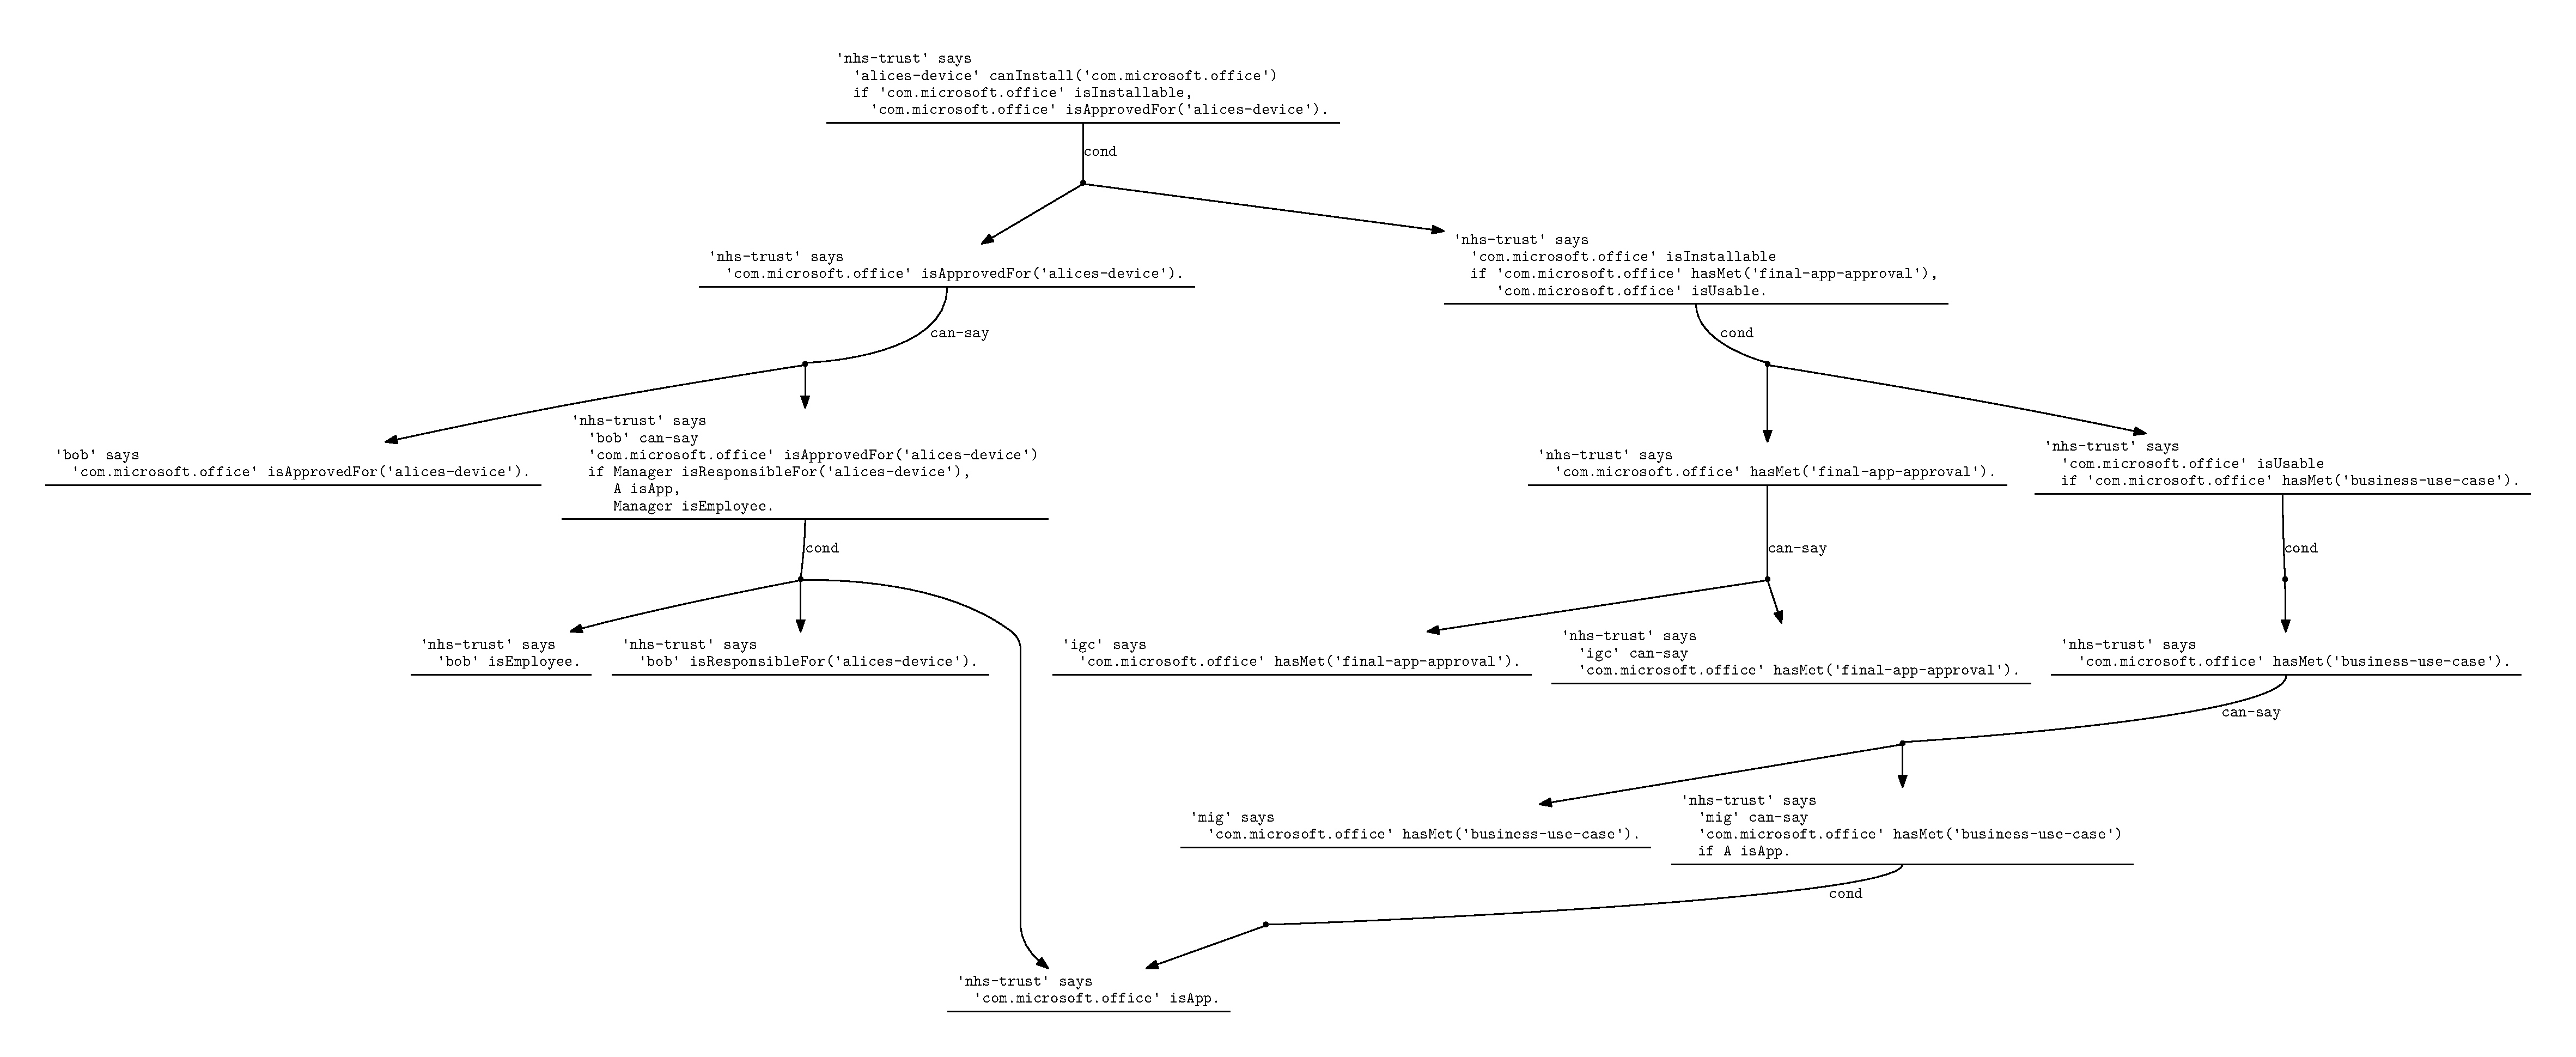
\includegraphics[width=1.0\textheight, angle=90]{figures/exemplar-proof.pdf}
  \caption[Proof tree output by AppPAL]{Proof tree generated by AppPAL when checking whether to install Alice's app.}
  \label{fig:exemplar-proof}
\end{figure}

\section{Implementation}
\label{sec:implementation}

The AppPAL implementation is a Java library, with roughly 5,000 lines of code.
The implementation is available online\footnote{\url{https://github.com/apppal/libapppal}}.
The library creates an AppPAL instance.
This instance can be given several policies to enforce (\autoref{fig:apppal-inputs-outputs}).
The instance is queried and will give decisions based on whether the queried assertion is valid according to the policy.
As part of the constraint checking AppPAL can also be connected to external databases, systems, and static analysis tools.
These can give AppPAL with more information external to that provided by SecPAL at the time of checking.

Implementing AppPAL as a library allows us to embed into a variety of situations.
It can be part of an app store checking the apps sold against a policy.
Running on a device it can check apps before installation by the package manager.
There is also a command-line version which is useful for testing and modelling policies.

The AppPAL interpreter implements SecPAL's evaluation rules (shown in~\autoref{fig:secpal-rules}) directly.
This differs from Becker's original description of SecPAL~\cite{becker_secpal:_2010} which describes evaluation through Datalog$^C$.
Datalog$^C$ is Datalog extended to support constraints~\cite{li_datalog_2003}.
Rather than implementing Datalog$^C$ and then AppPAL atop it (we could not find an existing implementation), AppPAL implements the evaluation rules directly.
This allows greater control over when AppPAL caches results, which is important in memory-constrained mobile devices.

\begin{figure}
  \centering
  \begin{eqnarray*}
    \infer[\textsf{\scriptsize cond}]{%
      AC, D \models A\textsf{~says~}fact\theta
    }{%
      \begin{array}[c]{c}
        \left(A\textsf{~says~}\textit{fact}\textsf{~if~}\textit{fact}_1, \ldots, \textit{fact}_k, c\right) \in AC \\
        AC,D\models A\textsf{~says~}\textit{fact}_i\theta \; \forall i \in \{1\cdots k\}
      \end{array}
      & \models{c\theta}
      & \textsf{vars}(\textit{fact}\theta) = \emptyset)
    }\\
    \infer[\textsf{\scriptsize can say}]{%
      AC, \infty \models A\textsf{~says~}\textit{fact}
    }{%
      AC, \infty \models A\textsf{~says~}B\textsf{~can~say}_D \textit{fact}
      & AC, D \models B\textsf{~says~}\textit{fact}
    } \\
    \infer[\textsf{\scriptsize can act as}]{%
      AC, D \models A\textsf{~says~}B~\textit{verbphrase}
    }{%
      AC, D \models A\textsf{~says~}B\textsf{~can~act~as~}C
      & AC, D \models A\textsf{~says~}C~\textit{verbphrase}
    }
  \end{eqnarray*}
  \caption[Inference rules used to evaluate {SecPAL}.]{The inference rules used to evaluate {SecPAL}. All {SecPAL} rules are
  evaluated in the context of a set of other assertions $AC$ as well as an
  allowed level of delegation $D$ which may be $0$ or $\infty$.}
\label{fig:secpal-rules}
\end{figure}

\begin{figure}
  \centering
  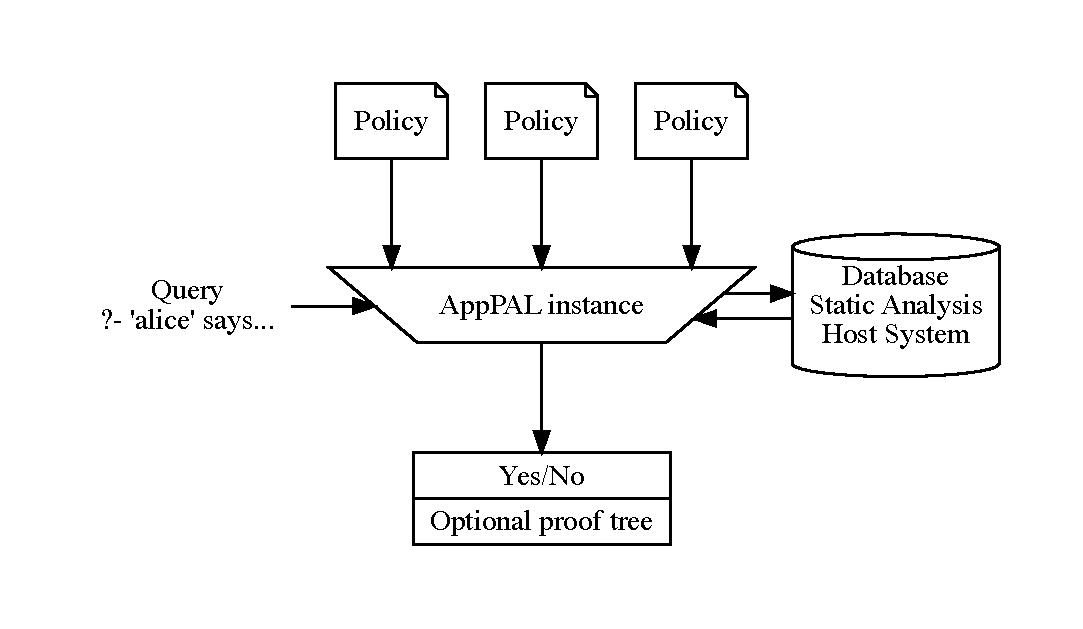
\includegraphics[width=\linewidth]{figures/apppal-evaluation.pdf}
  \caption{AppPAL's inputs and outputs}
  \label{fig:apppal-inputs-outputs}
\end{figure}

\subsection{Evaluation}
\label{ssec:evaluation-alg}

Pseudocode for AppPAL's evaluation algorithm is given in Algorithms~\cref{alg:eval1,alg:eval2,alg:eval3}.

To make queries against a policy AppPAL is first given one or more policy files.
AppPAL parses the files and adds the assertions within them to the \ac{AC}.
The AC is then preprocessed to extract more information; summarized in \autoref{tab:apppal-sets}.
If a constant is used before a \emph{says} statement, or it is used as the subject of a \emph{can-say} fact then the constant is marked as \emph{voiced}.
A constant is \emph{voiced} if it is the speaker of a statement or it is the subject of a \emph{can-say} fact.
A constant is a \emph{subject} is it is the subject of a fact.
The predicates used in the policy are also extracted and marked as \emph{derivable}.
This allows some queries to be decided automatically and some rules to be flagged as unusable in the assertion context.
This lets AppPAL reject some queries quickly: if they have a speaker that isn't voiced then we cannot query what they say.
If a rule relies on un-derivable predicates then it cannot be used to make decisions.

A results table is also created.
All ground facts in the assertion context are added to the results table as proven facts.
The table stores partial results and previously established proofs.
The table is indexed by queries and a delegation depth, partial results (i.e. that the evaluation of this query is ongoing).
This allows previous results to reused without re-computation or constraint re-evaluation.
It also prevents AppPAL proofs growing infinite in size (and the decision process not terminating).
If when searching for a proof we meet a query that we are currently evaluating, i.e.~one that exists higher in the current proof tree, we treat it as false.
Multiple queries will share the same results table until the table is cleared, or the AppPAL instance is stopped.

When evaluating the policy we also track which rules and predicates we have used.
From this we can reconstruct a proof tree that shows how AppPAL made a decision.
This allows an auditor to check the decision-making process and aids AppPAL's developers with debugging.

\begin{table}
  \centering
  \newcommand{\myset}[1]{\ensuremath{\text{\sffamily #1}}}
  \begin{tabular}{r l c}
    \toprule
    $c \in \myset{Voiced} \impliedby$     & $\exists \left(c \text{~says~} \cdots\right) \in \text{AC}$                        & $\bigvee$ \\
                                          & $\exists \left(\star \text{~says~} c \text{~can-say~} \cdots\right) \in \text{AC}$ &           \\
    $c \in \myset{Subjects} \impliedby$   & $\exists \left(\star \text{~says~} c\cdots\right) \in \text{AC}$                   & $\bigvee$ \\
                                          & $\exists \left(\cdots \text{~if~} \cdots,c~\star,\cdots\right) \in \text{AC},$     &           \\
                                          & $c \in \myset{Constants}$                                                          &           \\
    $p \in \myset{Derivable} \impliedby$  & $\exists \left( \cdots \star~p\left(\cdots\right) \cdots\right) \in \text{AC}$     &           \\
    \bottomrule                          \\
  \end{tabular}
  \caption{Sets used in AppPAL evaluation.}
  \label{tab:apppal-sets}
\end{table}

\begin{algorithm}
  \Fn(){\FnEvaluate{AC, Results Table, Query, D}}{
    \If{Results Table.\FnContains{(Query, D)}}{
      result $\gets$ {Results Table.\FnGet{(Query, D)}}\;
      \If{result.\FnValid{}}{
        \Return Result
      }
      \Else{
        \Return{Failure}
      }
    }
    \Else{
      Results Table.\FnSet{(Query, D), (Inprogress, p)}\;
      p $\gets$ \FnCond{AC, Results Table, Query, D}\;
      \If{p.\FnValid{}}{
        Results Table.\FnSet{(Query, D), (Proven, p)}\;
        \Return{(Proven, p)}\;
      }
      \Else{
        p $\gets$ \FnCanSayCanActAs{AC, Results Table, Query, D}\;
        \If{p.\FnValid{}}{
          Results Table.\FnSet{(Query, D), (Proven, p)}\;
          \Return{(Proven, p)}\;
        }
        \Else{
          Results Table.\FnSet{(Query, D), Failure}\;
          \Return{Failure}\;
        }
      }
    }
  }
  \caption{Pseudocode for evaluating a query.}
  \label{alg:eval1}
\end{algorithm}
\begin{algorithm}
  \ContinuedFloat
  \Fn(){\FnCanSayCanActAs{AC, Results Table, Query, D}}{
    \For{c $\in$ \FnConstants{AC}}{
      \If{c $\in$ \FnSubjects{AC}}{
        p $\gets$ \FnCanActAs{AC, Results Table, Query, D}\;
        \If{p.\FnValid{}}{\Return p}
      }
      \If{c $\in$ \FnSpeakers{AC}}{
        p $\gets$ \FnCanSay{AC, Results Table, Query, D}\;
        \If{p.\FnValid{}}{\Return p}
      }
    }
    \Return{Failure}
  }
  \caption{Pseudocode for using the can-say and can-act-as rules.}
  \label{alg:eval2}
\end{algorithm}
\begin{algorithm}
  \ContinuedFloat
  \Fn(){\FnCond{AC, Results Table, Query, D}}{
    \For{a $\in$ \FnAssertions{AC}}{
      u $\gets$ Query.\FnUnify{a.\FnHead{}}\;
      \If{u.\FnValid{}}{
        a $\gets$ a.\FnApply{u}
        \If{\FnVariables{a} = $\emptyset$}{
          \Return{\FnCheckBody{AC, Results Table, a, D}}
          \For{$\theta \in$ \FnVarSubs{AC, Assertion}}{
            a$^\prime$ $\gets$ a.\FnApply{$\theta$}\;
            \If{$\forall$ b $\in$ a$^\prime$.\FnBody{}: \FnEvaluate{AC, Results Table, b, D}.\FnValid{}}{
              p $\gets$ \FnCheckConstraint{a$^\prime$.\FnConstraint{}}\;
              \If{p.\FnValid{}}{\Return{p}}
            }
          }
        }
      }
    }
    \Return{Failure}
  }
    \caption{Pseudocode for using the cond-rule.}
    \label{alg:eval3}
\end{algorithm}

%\subsection{Correctness/Complexity}
%\todo{You know you're going to have to do this.}

\subsection{Benchmarks}
\label{ssec:benchmarks}

Someone using AppPAL might wish it to check apps before installation.
Since policy checks may involve inspecting many rules and constraints one may ask whether the checking will be acceptably fast.
Downloading and installing an app takes about 30 seconds on a typical Android phone over Wifi.
If checking a policy delays this even further a user may become annoyed and disable AppPAL.

A synthetic benchmark is used to give a measure AppPAL's performance.
The policy checking procedure is at its slowest when having to delegate repeatedly;
  the depth of the delegation tree is the biggest reason for slowing the search.
Synthetic benchmarks checks that the checking procedure performed acceptably.
Each benchmark consisted of a chain of delegations.
The \emph{1 to 1} benchmark consists of a repeated delegation between all the principals.
In the \emph{1 to 2} benchmark each principal delegated to 2 others and in the \emph{1 to 3} benchmark each principal delegated to 3 others.
These benchmarks are reasonable as they model the slowest kinds of policies to test---though worse ones could be designed by delegating even more or triggering an expensive constraint check.

\noindent
\begin{minipage}{.30\textwidth}
\begin{lstlisting}[caption={Excerpt of policy from 1 to 1 benchmark.}, basicstyle=\ttfamily\footnotesize]
'0' says '1' can-say
  X isInstallable.
'1' says '2' can-say
  X isInstallable.
'2' says '3' can-say
  X isInstallable.
\end{lstlisting}
\end{minipage}\hfill
\begin{minipage}{.30\textwidth}
\begin{lstlisting}[caption={Excerpt of policy from 1 to 2 benchmark.}, basicstyle=\ttfamily\footnotesize]
'2' says '4' can-say
  X isInstallable.
'2' says '5' can-say
  X isInstallable.
'3' says '6' can-say
  X isInstallable.
'3' says '7' can-say
  X isInstallable.
\end{lstlisting}
\end{minipage}\hfill
\begin{minipage}{.30\textwidth}
\begin{lstlisting}[caption={Excerpt of policy from 1 to 3 benchmark.}, basicstyle=\ttfamily\footnotesize]
'4' says '12' can-say
  X isInstallable.
'4' says '13' can-say
  X isInstallable.
'4' says '14' can-say
  X isInstallable.
'5' says '15' can-say
  X isInstallable.
'5' says '16' can-say
  X isInstallable.
'5' says '17' can-say
  X isInstallable.
\end{lstlisting}
\end{minipage}

For each benchmark we controlled the number of principals in the policy file:
as the number of principals increased so did the size of the policy.
The results are shown in \autoref{tab:benchmarks}.
Most typical policies (such as those discussed in \autoref{chap:apps-and-stores} and \autoref{chap:byod}), use only few delegations per decision.
I believe the policy checking performance of AppPAL is acceptable as unless a policy consists of hundreds of delegating principals the overhead of checking an AppPAL policy is negligible, even on a power constrained device such as a mobile phone~\cite{hallett_apppal_2016}.

\begin{table}
  \centering\sffamily
    \begin{tabular}{c c r@{.}l}
      \toprule
      Delegations & Principals & \multicolumn{2}{c}{Time (s)} \\
      \midrule
      1 to 1 & 10   &  0&01 \\
      1 to 1 & 100  &  1&00 \\
      1 to 1 & 500  & 20&90 \\
      1 to 1 & 1000 & 88&73 \\
      \midrule
      1 to 2 & 10   &  0&01 \\
      1 to 2 & 100  &  0&43 \\
      1 to 2 & 500  &  7&36 \\
      1 to 2 & 1000 & 27&47 \\
      \midrule
      1 to 3 & 10   &  0&01 \\
      1 to 3 & 100  &  0&24 \\
      1 to 3 & 500  &  3&99 \\
      1 to 3 & 1000 & 15&28 \\
      \bottomrule
    \end{tabular}
    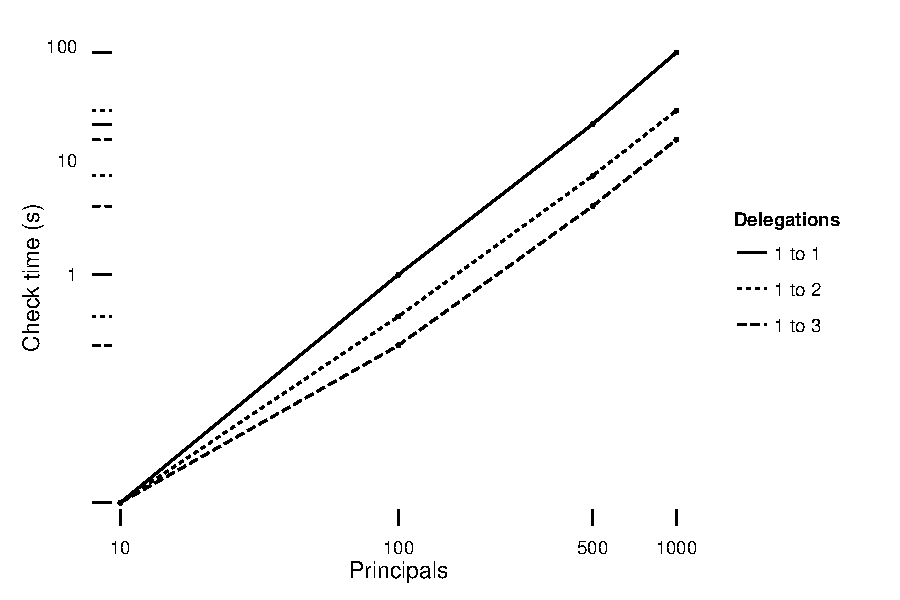
\includegraphics[width=1.00\linewidth]{figures/benchmarks.pdf}
  \caption{Benchmarking results on a Nexus 4 Android phone.}
  \label{tab:benchmarks}
\end{table}



\ignore{
  \bibliography{../thesis.bib}
}
\end{document}

% vim: set makeprg=make\ ch3.pdf:

%%% Local Variables:
%%% mode: latex
%%% TeX-master: "../ch3.tex"
%%% End:
